\documentclass[1p]{elsarticle_modified}
%\bibliographystyle{elsarticle-num}

%\usepackage[colorlinks]{hyperref}
%\usepackage{abbrmath_seonhwa} %\Abb, \Ascr, \Acal ,\Abf, \Afrak
\usepackage{amsfonts}
\usepackage{amssymb}
\usepackage{amsmath}
\usepackage{amsthm}
\usepackage{scalefnt}
\usepackage{amsbsy}
\usepackage{kotex}
\usepackage{caption}
\usepackage{subfig}
\usepackage{color}
\usepackage{graphicx}
\usepackage{xcolor} %% white, black, red, green, blue, cyan, magenta, yellow
\usepackage{float}
\usepackage{setspace}
\usepackage{hyperref}

\usepackage{tikz}
\usetikzlibrary{arrows}

\usepackage{multirow}
\usepackage{array} % fixed length table
\usepackage{hhline}

%%%%%%%%%%%%%%%%%%%%%
\makeatletter
\renewcommand*\env@matrix[1][\arraystretch]{%
	\edef\arraystretch{#1}%
	\hskip -\arraycolsep
	\let\@ifnextchar\new@ifnextchar
	\array{*\c@MaxMatrixCols c}}
\makeatother %https://tex.stackexchange.com/questions/14071/how-can-i-increase-the-line-spacing-in-a-matrix
%%%%%%%%%%%%%%%

\usepackage[normalem]{ulem}

\newcommand{\msout}[1]{\ifmmode\text{\sout{\ensuremath{#1}}}\else\sout{#1}\fi}
%SOURCE: \msout is \stkout macro in https://tex.stackexchange.com/questions/20609/strikeout-in-math-mode

\newcommand{\cancel}[1]{
	\ifmmode
	{\color{red}\msout{#1}}
	\else
	{\color{red}\sout{#1}}
	\fi
}

\newcommand{\add}[1]{
	{\color{blue}\uwave{#1}}
}

\newcommand{\replace}[2]{
	\ifmmode
	{\color{red}\msout{#1}}{\color{blue}\uwave{#2}}
	\else
	{\color{red}\sout{#1}}{\color{blue}\uwave{#2}}
	\fi
}

\newcommand{\Sol}{\mathcal{S}} %segment
\newcommand{\D}{D} %diagram
\newcommand{\A}{\mathcal{A}} %arc


%%%%%%%%%%%%%%%%%%%%%%%%%%%%%5 test

\def\sl{\operatorname{\textup{SL}}(2,\Cbb)}
\def\psl{\operatorname{\textup{PSL}}(2,\Cbb)}
\def\quan{\mkern 1mu \triangleright \mkern 1mu}

\theoremstyle{definition}
\newtheorem{thm}{Theorem}[section]
\newtheorem{prop}[thm]{Proposition}
\newtheorem{lem}[thm]{Lemma}
\newtheorem{ques}[thm]{Question}
\newtheorem{cor}[thm]{Corollary}
\newtheorem{defn}[thm]{Definition}
\newtheorem{exam}[thm]{Example}
\newtheorem{rmk}[thm]{Remark}
\newtheorem{alg}[thm]{Algorithm}

\newcommand{\I}{\sqrt{-1}}
\begin{document}

%\begin{frontmatter}
%
%\title{Boundary parabolic representations of knots up to 8 crossings}
%
%%% Group authors per affiliation:
%\author{Yunhi Cho} 
%\address{Department of Mathematics, University of Seoul, Seoul, Korea}
%\ead{yhcho@uos.ac.kr}
%
%
%\author{Seonhwa Kim} %\fnref{s_kim}}
%\address{Center for Geometry and Physics, Institute for Basic Science, Pohang, 37673, Korea}
%\ead{ryeona17@ibs.re.kr}
%
%\author{Hyuk Kim}
%\address{Department of Mathematical Sciences, Seoul National University, Seoul 08826, Korea}
%\ead{hyukkim@snu.ac.kr}
%
%\author{Seokbeom Yoon}
%\address{Department of Mathematical Sciences, Seoul National University, Seoul, 08826,  Korea}
%\ead{sbyoon15@snu.ac.kr}
%
%\begin{abstract}
%We find all boundary parabolic representation of knots up to 8 crossings.
%
%\end{abstract}
%\begin{keyword}
%    \MSC[2010] 57M25 
%\end{keyword}
%
%\end{frontmatter}

%\linenumbers
%\tableofcontents
%
\newcommand\colored[1]{\textcolor{white}{\rule[-0.35ex]{0.8em}{1.4ex}}\kern-0.8em\color{red} #1}%
%\newcommand\colored[1]{\textcolor{white}{ #1}\kern-2.17ex	\textcolor{white}{ #1}\kern-1.81ex	\textcolor{white}{ #1}\kern-2.15ex\color{red}#1	}

{\Large $\underline{11a_{322}~(K11a_{322})}$}

\setlength{\tabcolsep}{10pt}
\renewcommand{\arraystretch}{1.6}
\vspace{1cm}\begin{tabular}{m{100pt}>{\centering\arraybackslash}m{274pt}}
\multirow{5}{120pt}{
	\centering
	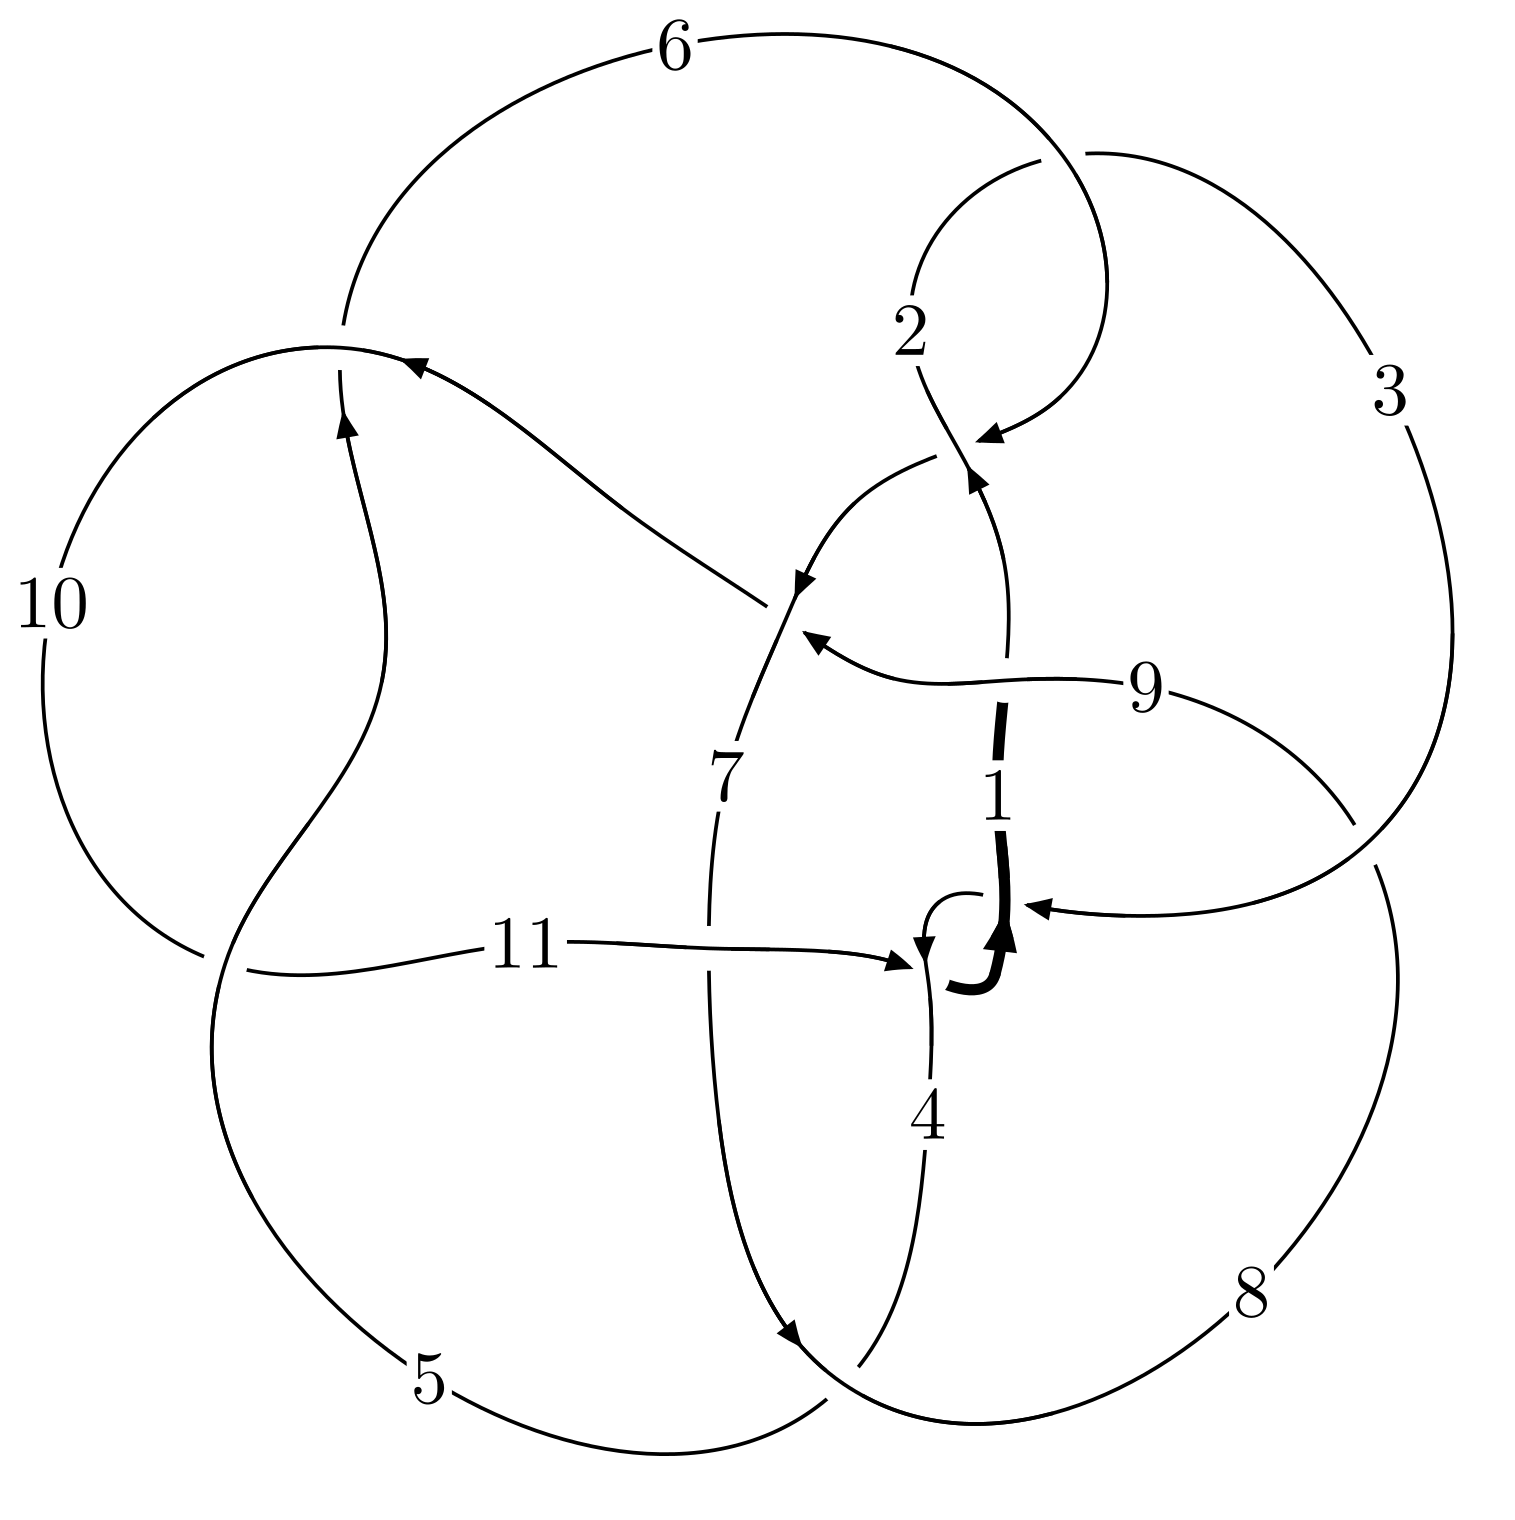
\includegraphics[width=112pt]{../../../GIT/diagram.site/Diagrams/png/571_11a_322.png}\\
\ \ \ A knot diagram\footnotemark}&
\allowdisplaybreaks
\textbf{Linearized knot diagam} \\
\cline{2-2}
 &
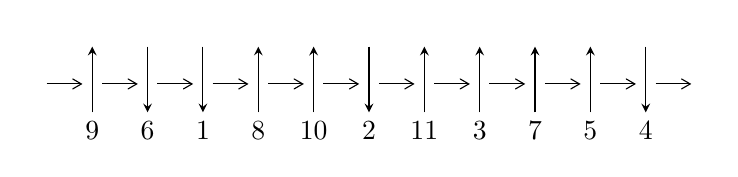
\begin{tikzpicture}[x=20pt, y=17pt]
	% nodes
	\node (C0) at (0, 0) {};
	\node (C1) at (1, 0) {};
	\node (C1U) at (1, +1) {};
	\node (C1D) at (1, -1) {9};

	\node (C2) at (2, 0) {};
	\node (C2U) at (2, +1) {};
	\node (C2D) at (2, -1) {6};

	\node (C3) at (3, 0) {};
	\node (C3U) at (3, +1) {};
	\node (C3D) at (3, -1) {1};

	\node (C4) at (4, 0) {};
	\node (C4U) at (4, +1) {};
	\node (C4D) at (4, -1) {8};

	\node (C5) at (5, 0) {};
	\node (C5U) at (5, +1) {};
	\node (C5D) at (5, -1) {10};

	\node (C6) at (6, 0) {};
	\node (C6U) at (6, +1) {};
	\node (C6D) at (6, -1) {2};

	\node (C7) at (7, 0) {};
	\node (C7U) at (7, +1) {};
	\node (C7D) at (7, -1) {11};

	\node (C8) at (8, 0) {};
	\node (C8U) at (8, +1) {};
	\node (C8D) at (8, -1) {3};

	\node (C9) at (9, 0) {};
	\node (C9U) at (9, +1) {};
	\node (C9D) at (9, -1) {7};

	\node (C10) at (10, 0) {};
	\node (C10U) at (10, +1) {};
	\node (C10D) at (10, -1) {5};

	\node (C11) at (11, 0) {};
	\node (C11U) at (11, +1) {};
	\node (C11D) at (11, -1) {4};
	\node (C12) at (12, 0) {};

	% arrows
	\draw[->,>={angle 60}]
	(C0) edge (C1) (C1) edge (C2) (C2) edge (C3) (C3) edge (C4) (C4) edge (C5) (C5) edge (C6) (C6) edge (C7) (C7) edge (C8) (C8) edge (C9) (C9) edge (C10) (C10) edge (C11) (C11) edge (C12) ;	\draw[->,>=stealth]
	(C1D) edge (C1U) (C2U) edge (C2D) (C3U) edge (C3D) (C4D) edge (C4U) (C5D) edge (C5U) (C6U) edge (C6D) (C7D) edge (C7U) (C8D) edge (C8U) (C9D) edge (C9U) (C10D) edge (C10U) (C11U) edge (C11D) ;
	\end{tikzpicture} \\
\hhline{~~} \\& 
\textbf{Solving Sequence} \\ \cline{2-2} 
 &
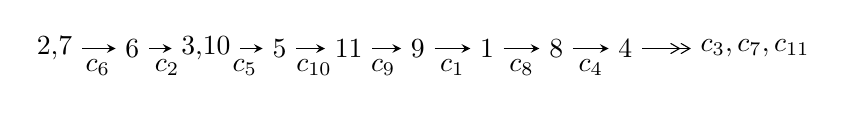
\begin{tikzpicture}[x=25pt, y=7pt]
	% node
	\node (A0) at (-1/8, 0) {2,7};
	\node (A1) at (1, 0) {6};
	\node (A2) at (33/16, 0) {3,10};
	\node (A3) at (25/8, 0) {5};
	\node (A4) at (33/8, 0) {11};
	\node (A5) at (41/8, 0) {9};
	\node (A6) at (49/8, 0) {1};
	\node (A7) at (57/8, 0) {8};
	\node (A8) at (65/8, 0) {4};
	\node (C1) at (1/2, -1) {$c_{6}$};
	\node (C2) at (3/2, -1) {$c_{2}$};
	\node (C3) at (21/8, -1) {$c_{5}$};
	\node (C4) at (29/8, -1) {$c_{10}$};
	\node (C5) at (37/8, -1) {$c_{9}$};
	\node (C6) at (45/8, -1) {$c_{1}$};
	\node (C7) at (53/8, -1) {$c_{8}$};
	\node (C8) at (61/8, -1) {$c_{4}$};
	\node (A9) at (10, 0) {$c_{3},c_{7},c_{11}$};

	% edge
	\draw[->,>=stealth]	
	(A0) edge (A1) (A1) edge (A2) (A2) edge (A3) (A3) edge (A4) (A4) edge (A5) (A5) edge (A6) (A6) edge (A7) (A7) edge (A8) ;
	\draw[->>,>={angle 60}]	
	(A8) edge (A9);
\end{tikzpicture} \\ 

\end{tabular} \\

\footnotetext{
The image of knot diagram is generated by the software ``\textbf{Draw programme}" developed by Andrew Bartholomew(\url{http://www.layer8.co.uk/maths/draw/index.htm\#Running-draw}), where we modified some parts for our purpose(\url{https://github.com/CATsTAILs/LinksPainter}).
}\phantom \\ \newline 
\centering \textbf{Ideals for irreducible components\footnotemark of $X_{\text{par}}$} 
 
\begin{align*}
I^u_{1}&=\langle 
1.55718\times10^{218} u^{92}-5.35792\times10^{218} u^{91}+\cdots+2.85769\times10^{219} b+6.67281\times10^{220},\\
\phantom{I^u_{1}}&\phantom{= \langle  }-4.75826\times10^{220} u^{92}-1.96732\times10^{221} u^{91}+\cdots+2.65765\times10^{221} a-7.23028\times10^{221},\\
\phantom{I^u_{1}}&\phantom{= \langle  }u^{93}+3 u^{92}+\cdots+151 u-93\rangle \\
I^u_{2}&=\langle 
7565 u^{17}-6236 u^{16}+\cdots+1467 b-19294,\;7565 u^{17}-7703 u^{16}+\cdots+1467 a-22228,\\
\phantom{I^u_{2}}&\phantom{= \langle  }u^{18}+4 u^{16}+7 u^{14}+u^{13}+6 u^{12}+5 u^{11}+9 u^{10}+7 u^9+23 u^8+34 u^6-7 u^5+24 u^4-5 u^3+8 u^2- u+1\rangle \\
\\
\end{align*}
\raggedright * 2 irreducible components of $\dim_{\mathbb{C}}=0$, with total 111 representations.\\
\footnotetext{All coefficients of polynomials are rational numbers. But the coefficients are sometimes approximated in decimal forms when there is not enough margin.}
\newpage
\renewcommand{\arraystretch}{1}
\centering \section*{I. $I^u_{1}= \langle 1.56\times10^{218} u^{92}-5.36\times10^{218} u^{91}+\cdots+2.86\times10^{219} b+6.67\times10^{220},\;-4.76\times10^{220} u^{92}-1.97\times10^{221} u^{91}+\cdots+2.66\times10^{221} a-7.23\times10^{221},\;u^{93}+3 u^{92}+\cdots+151 u-93 \rangle$}
\flushleft \textbf{(i) Arc colorings}\\
\begin{tabular}{m{7pt} m{180pt} m{7pt} m{180pt} }
\flushright $a_{2}=$&$\begin{pmatrix}0\\u\end{pmatrix}$ \\
\flushright $a_{7}=$&$\begin{pmatrix}1\\0\end{pmatrix}$ \\
\flushright $a_{6}=$&$\begin{pmatrix}1\\- u^2\end{pmatrix}$ \\
\flushright $a_{3}=$&$\begin{pmatrix}- u\\u^3+u\end{pmatrix}$ \\
\flushright $a_{10}=$&$\begin{pmatrix}0.179040 u^{92}+0.740246 u^{91}+\cdots-38.9739 u+2.72055\\-0.0544910 u^{92}+0.187491 u^{91}+\cdots+0.717266 u-23.3504\end{pmatrix}$ \\
\flushright $a_{5}=$&$\begin{pmatrix}0.367272 u^{92}+1.08675 u^{91}+\cdots-47.4264 u-0.976846\\0.614416 u^{92}+1.58014 u^{91}+\cdots-148.829 u+65.0773\end{pmatrix}$ \\
\flushright $a_{11}=$&$\begin{pmatrix}0.368295 u^{92}+1.12010 u^{91}+\cdots-50.3896 u+18.6394\\-0.280113 u^{92}-0.773917 u^{91}+\cdots+81.2460 u-42.5382\end{pmatrix}$ \\
\flushright $a_{9}=$&$\begin{pmatrix}0.233531 u^{92}+0.552755 u^{91}+\cdots-39.6912 u+26.0709\\-0.0544910 u^{92}+0.187491 u^{91}+\cdots+0.717266 u-23.3504\end{pmatrix}$ \\
\flushright $a_{1}=$&$\begin{pmatrix}0.556184 u^{92}+1.87340 u^{91}+\cdots-89.5355 u-0.790115\\-0.0755262 u^{92}-0.326383 u^{91}+\cdots+1.89622 u+13.2151\end{pmatrix}$ \\
\flushright $a_{8}=$&$\begin{pmatrix}0.0206578 u^{92}+0.0640587 u^{91}+\cdots-3.41149 u+8.80765\\-0.0463030 u^{92}+0.166139 u^{91}+\cdots+6.87334 u-20.0300\end{pmatrix}$ \\
\flushright $a_{4}=$&$\begin{pmatrix}-0.0387270 u^{92}+0.417865 u^{91}+\cdots+95.5003 u-88.9739\\0.131928 u^{92}+0.259721 u^{91}+\cdots-44.1127 u+34.0669\end{pmatrix}$\\ \flushright $a_{4}=$&$\begin{pmatrix}-0.0387270 u^{92}+0.417865 u^{91}+\cdots+95.5003 u-88.9739\\0.131928 u^{92}+0.259721 u^{91}+\cdots-44.1127 u+34.0669\end{pmatrix}$\\&\end{tabular}
\flushleft \textbf{(ii) Obstruction class $= -1$}\\~\\
\flushleft \textbf{(iii) Cusp Shapes $= 1.62307 u^{92}+5.49035 u^{91}+\cdots-409.463 u+157.721$}\\~\\
\newpage\renewcommand{\arraystretch}{1}
\flushleft \textbf{(iv) u-Polynomials at the component}\newline \\
\begin{tabular}{m{50pt}|m{274pt}}
Crossings & \hspace{64pt}u-Polynomials at each crossing \\
\hline $$\begin{aligned}c_{1}\end{aligned}$$&$\begin{aligned}
&u^{93}-5 u^{92}+\cdots+72835 u-5673
\end{aligned}$\\
\hline $$\begin{aligned}c_{2},c_{6}\end{aligned}$$&$\begin{aligned}
&u^{93}+3 u^{92}+\cdots+151 u-93
\end{aligned}$\\
\hline $$\begin{aligned}c_{3},c_{11}\end{aligned}$$&$\begin{aligned}
&u^{93}-5 u^{92}+\cdots+201 u-7
\end{aligned}$\\
\hline $$\begin{aligned}c_{4}\end{aligned}$$&$\begin{aligned}
&u^{93}-5 u^{92}+\cdots+20 u-3
\end{aligned}$\\
\hline $$\begin{aligned}c_{5},c_{10}\end{aligned}$$&$\begin{aligned}
&u^{93}- u^{92}+\cdots-5563 u-397
\end{aligned}$\\
\hline $$\begin{aligned}c_{7}\end{aligned}$$&$\begin{aligned}
&u^{93}-2 u^{91}+\cdots-16 u-3
\end{aligned}$\\
\hline $$\begin{aligned}c_{8}\end{aligned}$$&$\begin{aligned}
&u^{93}+u^{92}+\cdots-588 u-239
\end{aligned}$\\
\hline $$\begin{aligned}c_{9}\end{aligned}$$&$\begin{aligned}
&u^{93}-7 u^{92}+\cdots-37161 u-16439
\end{aligned}$\\
\hline
\end{tabular}\\~\\
\newpage\renewcommand{\arraystretch}{1}
\flushleft \textbf{(v) Riley Polynomials at the component}\newline \\
\begin{tabular}{m{50pt}|m{274pt}}
Crossings & \hspace{64pt}Riley Polynomials at each crossing \\
\hline $$\begin{aligned}c_{1}\end{aligned}$$&$\begin{aligned}
&y^{93}-33 y^{92}+\cdots+1446332815 y-32182929
\end{aligned}$\\
\hline $$\begin{aligned}c_{2},c_{6}\end{aligned}$$&$\begin{aligned}
&y^{93}+51 y^{92}+\cdots+26707 y-8649
\end{aligned}$\\
\hline $$\begin{aligned}c_{3},c_{11}\end{aligned}$$&$\begin{aligned}
&y^{93}+69 y^{92}+\cdots+4155 y-49
\end{aligned}$\\
\hline $$\begin{aligned}c_{4}\end{aligned}$$&$\begin{aligned}
&y^{93}+3 y^{92}+\cdots+58 y-9
\end{aligned}$\\
\hline $$\begin{aligned}c_{5},c_{10}\end{aligned}$$&$\begin{aligned}
&y^{93}+65 y^{92}+\cdots-454143 y-157609
\end{aligned}$\\
\hline $$\begin{aligned}c_{7}\end{aligned}$$&$\begin{aligned}
&y^{93}-4 y^{92}+\cdots+94 y-9
\end{aligned}$\\
\hline $$\begin{aligned}c_{8}\end{aligned}$$&$\begin{aligned}
&y^{93}-17 y^{92}+\cdots-6001618 y-57121
\end{aligned}$\\
\hline $$\begin{aligned}c_{9}\end{aligned}$$&$\begin{aligned}
&y^{93}-9 y^{92}+\cdots+5192486461 y-270240721
\end{aligned}$\\
\hline
\end{tabular}\\~\\
\newpage\flushleft \textbf{(vi) Complex Volumes and Cusp Shapes}
$$\begin{array}{c|c|c}  
\text{Solutions to }I^u_{1}& \I (\text{vol} + \sqrt{-1}CS) & \text{Cusp shape}\\
 \hline 
\begin{aligned}
u &= \phantom{-}0.322622 + 0.930689 I \\
a &= -2.15336 + 0.73375 I \\
b &= -0.573278 + 0.461113 I\end{aligned}
 & -3.27973 - 4.30614 I & \phantom{-0.000000 } 0 \\ \hline\begin{aligned}
u &= \phantom{-}0.322622 - 0.930689 I \\
a &= -2.15336 - 0.73375 I \\
b &= -0.573278 - 0.461113 I\end{aligned}
 & -3.27973 + 4.30614 I & \phantom{-0.000000 } 0 \\ \hline\begin{aligned}
u &= -0.131902 + 0.954095 I \\
a &= -1.77797 - 0.58692 I \\
b &= -1.236380 + 0.556414 I\end{aligned}
 & \phantom{-}3.10875 + 0.58240 I & \phantom{-0.000000 } 0 \\ \hline\begin{aligned}
u &= -0.131902 - 0.954095 I \\
a &= -1.77797 + 0.58692 I \\
b &= -1.236380 - 0.556414 I\end{aligned}
 & \phantom{-}3.10875 - 0.58240 I & \phantom{-0.000000 } 0 \\ \hline\begin{aligned}
u &= -0.299211 + 0.900944 I \\
a &= \phantom{-}2.54722 + 1.40953 I \\
b &= \phantom{-}1.15602 + 1.37213 I\end{aligned}
 & \phantom{-}0.45952 - 4.22823 I & \phantom{-0.000000 } 0 \\ \hline\begin{aligned}
u &= -0.299211 - 0.900944 I \\
a &= \phantom{-}2.54722 - 1.40953 I \\
b &= \phantom{-}1.15602 - 1.37213 I\end{aligned}
 & \phantom{-}0.45952 + 4.22823 I & \phantom{-0.000000 } 0 \\ \hline\begin{aligned}
u &= -0.608017 + 0.715465 I \\
a &= \phantom{-}1.24868 - 1.08837 I \\
b &= \phantom{-}1.242490 - 0.457719 I\end{aligned}
 & -0.03049 + 2.41359 I & \phantom{-0.000000 } 0 \\ \hline\begin{aligned}
u &= -0.608017 - 0.715465 I \\
a &= \phantom{-}1.24868 + 1.08837 I \\
b &= \phantom{-}1.242490 + 0.457719 I\end{aligned}
 & -0.03049 - 2.41359 I & \phantom{-0.000000 } 0 \\ \hline\begin{aligned}
u &= \phantom{-}0.937372 + 0.000279 I \\
a &= -0.071937 - 0.342014 I \\
b &= \phantom{-}0.987401 + 0.314558 I\end{aligned}
 & \phantom{-}4.23878 + 6.45548 I & \phantom{-0.000000 } 0 \\ \hline\begin{aligned}
u &= \phantom{-}0.937372 - 0.000279 I \\
a &= -0.071937 + 0.342014 I \\
b &= \phantom{-}0.987401 - 0.314558 I\end{aligned}
 & \phantom{-}4.23878 - 6.45548 I & \phantom{-0.000000 } 0\\
 \hline 
 \end{array}$$\newpage$$\begin{array}{c|c|c}  
\text{Solutions to }I^u_{1}& \I (\text{vol} + \sqrt{-1}CS) & \text{Cusp shape}\\
 \hline 
\begin{aligned}
u &= \phantom{-}0.844094 + 0.653935 I \\
a &= \phantom{-}0.698181 + 0.068263 I \\
b &= -0.243081 + 0.556201 I\end{aligned}
 & -1.68544 - 3.00936 I & \phantom{-0.000000 } 0 \\ \hline\begin{aligned}
u &= \phantom{-}0.844094 - 0.653935 I \\
a &= \phantom{-}0.698181 - 0.068263 I \\
b &= -0.243081 - 0.556201 I\end{aligned}
 & -1.68544 + 3.00936 I & \phantom{-0.000000 } 0 \\ \hline\begin{aligned}
u &= \phantom{-}0.366246 + 0.856685 I \\
a &= \phantom{-}2.30851 - 0.38298 I \\
b &= \phantom{-}1.180700 - 0.617692 I\end{aligned}
 & -3.77658 + 0.38693 I & \phantom{-0.000000 } 0 \\ \hline\begin{aligned}
u &= \phantom{-}0.366246 - 0.856685 I \\
a &= \phantom{-}2.30851 + 0.38298 I \\
b &= \phantom{-}1.180700 + 0.617692 I\end{aligned}
 & -3.77658 - 0.38693 I & \phantom{-0.000000 } 0 \\ \hline\begin{aligned}
u &= -1.068810 + 0.000483 I \\
a &= \phantom{-}0.305136 - 0.317752 I \\
b &= -0.349343 - 0.764786 I\end{aligned}
 & -2.91806 + 1.82006 I & \phantom{-0.000000 } 0 \\ \hline\begin{aligned}
u &= -1.068810 - 0.000483 I \\
a &= \phantom{-}0.305136 + 0.317752 I \\
b &= -0.349343 + 0.764786 I\end{aligned}
 & -2.91806 - 1.82006 I & \phantom{-0.000000 } 0 \\ \hline\begin{aligned}
u &= -0.445066 + 0.987704 I \\
a &= -2.09200 - 0.52232 I \\
b &= -0.553513 - 1.003530 I\end{aligned}
 & -0.44062 + 9.04830 I & \phantom{-0.000000 } 0 \\ \hline\begin{aligned}
u &= -0.445066 - 0.987704 I \\
a &= -2.09200 + 0.52232 I \\
b &= -0.553513 + 1.003530 I\end{aligned}
 & -0.44062 - 9.04830 I & \phantom{-0.000000 } 0 \\ \hline\begin{aligned}
u &= -0.539921 + 0.940488 I \\
a &= \phantom{-}1.265850 + 0.049756 I \\
b &= \phantom{-}0.507207 + 0.197470 I\end{aligned}
 & -0.87942 + 2.94273 I & \phantom{-0.000000 } 0 \\ \hline\begin{aligned}
u &= -0.539921 - 0.940488 I \\
a &= \phantom{-}1.265850 - 0.049756 I \\
b &= \phantom{-}0.507207 - 0.197470 I\end{aligned}
 & -0.87942 - 2.94273 I & \phantom{-0.000000 } 0\\
 \hline 
 \end{array}$$\newpage$$\begin{array}{c|c|c}  
\text{Solutions to }I^u_{1}& \I (\text{vol} + \sqrt{-1}CS) & \text{Cusp shape}\\
 \hline 
\begin{aligned}
u &= \phantom{-}0.293670 + 1.064590 I \\
a &= -1.40531 - 0.46287 I \\
b &= -1.053630 + 0.748164 I\end{aligned}
 & \phantom{-}3.49041 - 2.34482 I & \phantom{-0.000000 } 0 \\ \hline\begin{aligned}
u &= \phantom{-}0.293670 - 1.064590 I \\
a &= -1.40531 + 0.46287 I \\
b &= -1.053630 - 0.748164 I\end{aligned}
 & \phantom{-}3.49041 + 2.34482 I & \phantom{-0.000000 } 0 \\ \hline\begin{aligned}
u &= -0.197477 + 0.859125 I \\
a &= -0.06670 - 1.86214 I \\
b &= \phantom{-}0.47109 - 2.64628 I\end{aligned}
 & \phantom{-}0.11047 + 6.51793 I & \phantom{-0.000000 } 0 \\ \hline\begin{aligned}
u &= -0.197477 - 0.859125 I \\
a &= -0.06670 + 1.86214 I \\
b &= \phantom{-}0.47109 + 2.64628 I\end{aligned}
 & \phantom{-}0.11047 - 6.51793 I & \phantom{-0.000000 } 0 \\ \hline\begin{aligned}
u &= -0.620927 + 0.950340 I \\
a &= -1.34145 + 1.19160 I \\
b &= -1.93676 - 0.00311 I\end{aligned}
 & \phantom{-}5.22424 + 2.46471 I & \phantom{-0.000000 } 0 \\ \hline\begin{aligned}
u &= -0.620927 - 0.950340 I \\
a &= -1.34145 - 1.19160 I \\
b &= -1.93676 + 0.00311 I\end{aligned}
 & \phantom{-}5.22424 - 2.46471 I & \phantom{-0.000000 } 0 \\ \hline\begin{aligned}
u &= -1.114510 + 0.270069 I \\
a &= -0.159734 - 0.487015 I \\
b &= \phantom{-}0.948829 - 0.853586 I\end{aligned}
 & \phantom{-}0.05288 - 11.48280 I & \phantom{-0.000000 } 0 \\ \hline\begin{aligned}
u &= -1.114510 - 0.270069 I \\
a &= -0.159734 + 0.487015 I \\
b &= \phantom{-}0.948829 + 0.853586 I\end{aligned}
 & \phantom{-}0.05288 + 11.48280 I & \phantom{-0.000000 } 0 \\ \hline\begin{aligned}
u &= -0.436496 + 1.069900 I \\
a &= -1.20356 + 0.86385 I \\
b &= -1.25197 - 0.90240 I\end{aligned}
 & \phantom{-}5.97802 + 3.41696 I & \phantom{-0.000000 } 0 \\ \hline\begin{aligned}
u &= -0.436496 - 1.069900 I \\
a &= -1.20356 - 0.86385 I \\
b &= -1.25197 + 0.90240 I\end{aligned}
 & \phantom{-}5.97802 - 3.41696 I & \phantom{-0.000000 } 0\\
 \hline 
 \end{array}$$\newpage$$\begin{array}{c|c|c}  
\text{Solutions to }I^u_{1}& \I (\text{vol} + \sqrt{-1}CS) & \text{Cusp shape}\\
 \hline 
\begin{aligned}
u &= \phantom{-}0.318884 + 0.770726 I \\
a &= \phantom{-}1.183980 + 0.175323 I \\
b &= -0.190440 - 0.528926 I\end{aligned}
 & \phantom{-}2.61018 + 0.55355 I & \phantom{-}5.97981 + 0. I\phantom{ +0.000000I} \\ \hline\begin{aligned}
u &= \phantom{-}0.318884 - 0.770726 I \\
a &= \phantom{-}1.183980 - 0.175323 I \\
b &= -0.190440 + 0.528926 I\end{aligned}
 & \phantom{-}2.61018 - 0.55355 I & \phantom{-}5.97981 + 0. I\phantom{ +0.000000I} \\ \hline\begin{aligned}
u &= \phantom{-}0.319146 + 0.760564 I \\
a &= \phantom{-}0.498308 + 1.151370 I \\
b &= \phantom{-}0.66734 + 1.64554 I\end{aligned}
 & -4.14473 - 3.51278 I & -1.54683 + 9.73709 I \\ \hline\begin{aligned}
u &= \phantom{-}0.319146 - 0.760564 I \\
a &= \phantom{-}0.498308 - 1.151370 I \\
b &= \phantom{-}0.66734 - 1.64554 I\end{aligned}
 & -4.14473 + 3.51278 I & -1.54683 - 9.73709 I \\ \hline\begin{aligned}
u &= \phantom{-}1.126650 + 0.344072 I \\
a &= \phantom{-}0.024805 + 0.458219 I \\
b &= \phantom{-}0.802756 + 0.733051 I\end{aligned}
 & -4.77635 + 5.74683 I & \phantom{-0.000000 } 0 \\ \hline\begin{aligned}
u &= \phantom{-}1.126650 - 0.344072 I \\
a &= \phantom{-}0.024805 - 0.458219 I \\
b &= \phantom{-}0.802756 - 0.733051 I\end{aligned}
 & -4.77635 - 5.74683 I & \phantom{-0.000000 } 0 \\ \hline\begin{aligned}
u &= -0.803406 + 0.165006 I \\
a &= \phantom{-}0.431389 - 0.253688 I \\
b &= -0.291133 - 0.942335 I\end{aligned}
 & -2.78159 + 1.95644 I & \phantom{-0.000000 } 0. - 2.42185 I \\ \hline\begin{aligned}
u &= -0.803406 - 0.165006 I \\
a &= \phantom{-}0.431389 + 0.253688 I \\
b &= -0.291133 + 0.942335 I\end{aligned}
 & -2.78159 - 1.95644 I & \phantom{-0.000000 -}0. + 2.42185 I \\ \hline\begin{aligned}
u &= \phantom{-}0.098315 + 0.812310 I \\
a &= -2.40378 - 0.73606 I \\
b &= -0.486771 + 0.372378 I\end{aligned}
 & \phantom{-}2.22253 - 2.87184 I & \phantom{-}5.92800 + 10.27307 I \\ \hline\begin{aligned}
u &= \phantom{-}0.098315 - 0.812310 I \\
a &= -2.40378 + 0.73606 I \\
b &= -0.486771 - 0.372378 I\end{aligned}
 & \phantom{-}2.22253 + 2.87184 I & \phantom{-}5.92800 - 10.27307 I\\
 \hline 
 \end{array}$$\newpage$$\begin{array}{c|c|c}  
\text{Solutions to }I^u_{1}& \I (\text{vol} + \sqrt{-1}CS) & \text{Cusp shape}\\
 \hline 
\begin{aligned}
u &= -0.263210 + 1.161530 I \\
a &= \phantom{-}0.745326 - 1.002680 I \\
b &= \phantom{-}0.436652 + 0.507867 I\end{aligned}
 & \phantom{-}4.67249 + 3.86717 I & \phantom{-0.000000 } 0 \\ \hline\begin{aligned}
u &= -0.263210 - 1.161530 I \\
a &= \phantom{-}0.745326 + 1.002680 I \\
b &= \phantom{-}0.436652 - 0.507867 I\end{aligned}
 & \phantom{-}4.67249 - 3.86717 I & \phantom{-0.000000 } 0 \\ \hline\begin{aligned}
u &= -1.102170 + 0.453309 I \\
a &= \phantom{-}0.344660 - 0.282026 I \\
b &= \phantom{-}0.587996 - 0.233648 I\end{aligned}
 & -1.79025 + 1.21167 I & \phantom{-0.000000 } 0 \\ \hline\begin{aligned}
u &= -1.102170 - 0.453309 I \\
a &= \phantom{-}0.344660 + 0.282026 I \\
b &= \phantom{-}0.587996 + 0.233648 I\end{aligned}
 & -1.79025 - 1.21167 I & \phantom{-0.000000 } 0 \\ \hline\begin{aligned}
u &= \phantom{-}0.374927 + 1.137660 I \\
a &= -0.449358 - 0.993803 I \\
b &= -1.033240 - 0.031958 I\end{aligned}
 & \phantom{-}5.66136 - 0.33582 I & \phantom{-0.000000 } 0 \\ \hline\begin{aligned}
u &= \phantom{-}0.374927 - 1.137660 I \\
a &= -0.449358 + 0.993803 I \\
b &= -1.033240 + 0.031958 I\end{aligned}
 & \phantom{-}5.66136 + 0.33582 I & \phantom{-0.000000 } 0 \\ \hline\begin{aligned}
u &= -0.172805 + 1.199490 I \\
a &= -1.60819 - 0.00472 I \\
b &= -1.55467 - 0.72808 I\end{aligned}
 & \phantom{-}8.09781 + 2.55341 I & \phantom{-0.000000 } 0 \\ \hline\begin{aligned}
u &= -0.172805 - 1.199490 I \\
a &= -1.60819 + 0.00472 I \\
b &= -1.55467 + 0.72808 I\end{aligned}
 & \phantom{-}8.09781 - 2.55341 I & \phantom{-0.000000 } 0 \\ \hline\begin{aligned}
u &= \phantom{-}0.067778 + 1.253000 I \\
a &= \phantom{-}0.686715 + 0.412175 I \\
b &= \phantom{-}0.469935 - 0.266987 I\end{aligned}
 & \phantom{-}2.03743 + 2.00663 I & \phantom{-0.000000 } 0 \\ \hline\begin{aligned}
u &= \phantom{-}0.067778 - 1.253000 I \\
a &= \phantom{-}0.686715 - 0.412175 I \\
b &= \phantom{-}0.469935 + 0.266987 I\end{aligned}
 & \phantom{-}2.03743 - 2.00663 I & \phantom{-0.000000 } 0\\
 \hline 
 \end{array}$$\newpage$$\begin{array}{c|c|c}  
\text{Solutions to }I^u_{1}& \I (\text{vol} + \sqrt{-1}CS) & \text{Cusp shape}\\
 \hline 
\begin{aligned}
u &= \phantom{-}0.723160 + 0.174661 I \\
a &= \phantom{-}0.836755 - 0.225299 I \\
b &= -0.761338 - 1.042850 I\end{aligned}
 & \phantom{-}1.92000 + 3.17965 I & \phantom{-}4.65573 - 4.19725 I \\ \hline\begin{aligned}
u &= \phantom{-}0.723160 - 0.174661 I \\
a &= \phantom{-}0.836755 + 0.225299 I \\
b &= -0.761338 + 1.042850 I\end{aligned}
 & \phantom{-}1.92000 - 3.17965 I & \phantom{-}4.65573 + 4.19725 I \\ \hline\begin{aligned}
u &= -0.403548 + 1.190460 I \\
a &= -0.364495 + 0.144692 I \\
b &= -0.418079 - 0.607354 I\end{aligned}
 & \phantom{-}1.44049 + 2.66870 I & \phantom{-0.000000 } 0 \\ \hline\begin{aligned}
u &= -0.403548 - 1.190460 I \\
a &= -0.364495 - 0.144692 I \\
b &= -0.418079 + 0.607354 I\end{aligned}
 & \phantom{-}1.44049 - 2.66870 I & \phantom{-0.000000 } 0 \\ \hline\begin{aligned}
u &= \phantom{-}0.261222 + 0.695240 I \\
a &= -0.225493 + 0.262106 I \\
b &= -0.276840 - 1.313040 I\end{aligned}
 & -4.08056 + 1.50596 I & \phantom{-}0.83759 + 2.64217 I \\ \hline\begin{aligned}
u &= \phantom{-}0.261222 - 0.695240 I \\
a &= -0.225493 - 0.262106 I \\
b &= -0.276840 + 1.313040 I\end{aligned}
 & -4.08056 - 1.50596 I & \phantom{-}0.83759 - 2.64217 I \\ \hline\begin{aligned}
u &= -0.707177 + 0.220909 I \\
a &= \phantom{-}0.511993 - 0.477897 I \\
b &= \phantom{-}0.437276 + 0.272075 I\end{aligned}
 & -1.39598 + 1.17736 I & -3.93052 - 4.80087 I \\ \hline\begin{aligned}
u &= -0.707177 - 0.220909 I \\
a &= \phantom{-}0.511993 + 0.477897 I \\
b &= \phantom{-}0.437276 - 0.272075 I\end{aligned}
 & -1.39598 - 1.17736 I & -3.93052 + 4.80087 I \\ \hline\begin{aligned}
u &= \phantom{-}0.504232 + 1.159730 I \\
a &= -1.99380 + 0.16893 I \\
b &= -1.55624 + 1.52324 I\end{aligned}
 & \phantom{-}4.76534 - 7.79767 I & \phantom{-0.000000 } 0 \\ \hline\begin{aligned}
u &= \phantom{-}0.504232 - 1.159730 I \\
a &= -1.99380 - 0.16893 I \\
b &= -1.55624 - 1.52324 I\end{aligned}
 & \phantom{-}4.76534 + 7.79767 I & \phantom{-0.000000 } 0\\
 \hline 
 \end{array}$$\newpage$$\begin{array}{c|c|c}  
\text{Solutions to }I^u_{1}& \I (\text{vol} + \sqrt{-1}CS) & \text{Cusp shape}\\
 \hline 
\begin{aligned}
u &= \phantom{-}0.346185 + 1.236500 I \\
a &= -0.702997 + 0.404800 I \\
b &= -0.464835 + 1.306190 I\end{aligned}
 & \phantom{-}4.73642 - 6.03450 I & \phantom{-0.000000 } 0 \\ \hline\begin{aligned}
u &= \phantom{-}0.346185 - 1.236500 I \\
a &= -0.702997 - 0.404800 I \\
b &= -0.464835 - 1.306190 I\end{aligned}
 & \phantom{-}4.73642 + 6.03450 I & \phantom{-0.000000 } 0 \\ \hline\begin{aligned}
u &= -0.504738 + 0.496846 I \\
a &= \phantom{-}0.289551 - 0.207560 I \\
b &= -0.28960 + 1.49053 I\end{aligned}
 & -1.87848 - 5.13684 I & \phantom{-}0.46607 + 1.98262 I \\ \hline\begin{aligned}
u &= -0.504738 - 0.496846 I \\
a &= \phantom{-}0.289551 + 0.207560 I \\
b &= -0.28960 - 1.49053 I\end{aligned}
 & -1.87848 + 5.13684 I & \phantom{-}0.46607 - 1.98262 I \\ \hline\begin{aligned}
u &= -0.463746 + 1.210540 I \\
a &= -1.68232 - 0.35122 I \\
b &= -1.33627 - 1.18381 I\end{aligned}
 & \phantom{-}0.97476 + 6.41730 I & \phantom{-0.000000 } 0 \\ \hline\begin{aligned}
u &= -0.463746 - 1.210540 I \\
a &= -1.68232 + 0.35122 I \\
b &= -1.33627 + 1.18381 I\end{aligned}
 & \phantom{-}0.97476 - 6.41730 I & \phantom{-0.000000 } 0 \\ \hline\begin{aligned}
u &= -0.416030 + 1.283650 I \\
a &= \phantom{-}1.279510 - 0.430873 I \\
b &= \phantom{-}0.913703 + 0.533909 I\end{aligned}
 & \phantom{-}3.10293 + 5.33107 I & \phantom{-0.000000 } 0 \\ \hline\begin{aligned}
u &= -0.416030 - 1.283650 I \\
a &= \phantom{-}1.279510 + 0.430873 I \\
b &= \phantom{-}0.913703 - 0.533909 I\end{aligned}
 & \phantom{-}3.10293 - 5.33107 I & \phantom{-0.000000 } 0 \\ \hline\begin{aligned}
u &= \phantom{-}0.485082 + 1.270200 I \\
a &= \phantom{-}1.286330 + 0.485594 I \\
b &= \phantom{-}1.140580 - 0.783321 I\end{aligned}
 & \phantom{-}8.11494 - 11.47080 I & \phantom{-0.000000 } 0 \\ \hline\begin{aligned}
u &= \phantom{-}0.485082 - 1.270200 I \\
a &= \phantom{-}1.286330 - 0.485594 I \\
b &= \phantom{-}1.140580 + 0.783321 I\end{aligned}
 & \phantom{-}8.11494 + 11.47080 I & \phantom{-0.000000 } 0\\
 \hline 
 \end{array}$$\newpage$$\begin{array}{c|c|c}  
\text{Solutions to }I^u_{1}& \I (\text{vol} + \sqrt{-1}CS) & \text{Cusp shape}\\
 \hline 
\begin{aligned}
u &= \phantom{-}0.318984 + 1.325490 I \\
a &= -1.49667 + 0.72618 I \\
b &= -1.52310 + 1.21358 I\end{aligned}
 & \phantom{-}4.36272 - 6.42244 I & \phantom{-0.000000 } 0 \\ \hline\begin{aligned}
u &= \phantom{-}0.318984 - 1.325490 I \\
a &= -1.49667 - 0.72618 I \\
b &= -1.52310 - 1.21358 I\end{aligned}
 & \phantom{-}4.36272 + 6.42244 I & \phantom{-0.000000 } 0 \\ \hline\begin{aligned}
u &= \phantom{-}0.454840 + 1.316880 I \\
a &= \phantom{-}1.067410 + 0.460691 I \\
b &= \phantom{-}1.218720 - 0.165295 I\end{aligned}
 & \phantom{-}8.34403 + 1.38464 I & \phantom{-0.000000 } 0 \\ \hline\begin{aligned}
u &= \phantom{-}0.454840 - 1.316880 I \\
a &= \phantom{-}1.067410 - 0.460691 I \\
b &= \phantom{-}1.218720 + 0.165295 I\end{aligned}
 & \phantom{-}8.34403 - 1.38464 I & \phantom{-0.000000 } 0 \\ \hline\begin{aligned}
u &= -0.537415 + 0.281055 I \\
a &= \phantom{-}1.260790 - 0.030814 I \\
b &= -0.910843 + 0.095195 I\end{aligned}
 & \phantom{-}3.79529 + 0.46350 I & \phantom{-}6.87686 - 1.81955 I \\ \hline\begin{aligned}
u &= -0.537415 - 0.281055 I \\
a &= \phantom{-}1.260790 + 0.030814 I \\
b &= -0.910843 - 0.095195 I\end{aligned}
 & \phantom{-}3.79529 - 0.46350 I & \phantom{-}6.87686 + 1.81955 I \\ \hline\begin{aligned}
u &= \phantom{-}1.286610 + 0.581347 I \\
a &= -0.050685 - 0.472761 I \\
b &= -0.587209 - 0.338343 I\end{aligned}
 & -2.62056 - 2.77773 I & \phantom{-0.000000 } 0 \\ \hline\begin{aligned}
u &= \phantom{-}1.286610 - 0.581347 I \\
a &= -0.050685 + 0.472761 I \\
b &= -0.587209 + 0.338343 I\end{aligned}
 & -2.62056 + 2.77773 I & \phantom{-0.000000 } 0 \\ \hline\begin{aligned}
u &= \phantom{-}0.64633 + 1.26191 I \\
a &= \phantom{-}1.50927 + 0.08635 I \\
b &= \phantom{-}1.32829 - 0.92505 I\end{aligned}
 & -1.80023 - 12.03950 I & \phantom{-0.000000 } 0 \\ \hline\begin{aligned}
u &= \phantom{-}0.64633 - 1.26191 I \\
a &= \phantom{-}1.50927 - 0.08635 I \\
b &= \phantom{-}1.32829 + 0.92505 I\end{aligned}
 & -1.80023 + 12.03950 I & \phantom{-0.000000 } 0\\
 \hline 
 \end{array}$$\newpage$$\begin{array}{c|c|c}  
\text{Solutions to }I^u_{1}& \I (\text{vol} + \sqrt{-1}CS) & \text{Cusp shape}\\
 \hline 
\begin{aligned}
u &= -0.63602 + 1.27863 I \\
a &= \phantom{-}1.61271 - 0.05318 I \\
b &= \phantom{-}1.51527 + 1.12304 I\end{aligned}
 & \phantom{-}3.2415 + 17.6972 I & \phantom{-0.000000 } 0 \\ \hline\begin{aligned}
u &= -0.63602 - 1.27863 I \\
a &= \phantom{-}1.61271 + 0.05318 I \\
b &= \phantom{-}1.51527 - 1.12304 I\end{aligned}
 & \phantom{-}3.2415 - 17.6972 I & \phantom{-0.000000 } 0 \\ \hline\begin{aligned}
u &= -0.64483 + 1.27730 I \\
a &= \phantom{-}1.322000 - 0.207651 I \\
b &= \phantom{-}1.149910 + 0.457616 I\end{aligned}
 & \phantom{-}1.14741 + 5.18553 I & \phantom{-0.000000 } 0 \\ \hline\begin{aligned}
u &= -0.64483 - 1.27730 I \\
a &= \phantom{-}1.322000 + 0.207651 I \\
b &= \phantom{-}1.149910 - 0.457616 I\end{aligned}
 & \phantom{-}1.14741 - 5.18553 I & \phantom{-0.000000 } 0 \\ \hline\begin{aligned}
u &= \phantom{-}0.75806 + 1.21920 I \\
a &= -1.019030 - 0.222304 I \\
b &= -1.169210 + 0.601044 I\end{aligned}
 & -0.38282 - 4.43447 I & \phantom{-0.000000 } 0 \\ \hline\begin{aligned}
u &= \phantom{-}0.75806 - 1.21920 I \\
a &= -1.019030 + 0.222304 I \\
b &= -1.169210 - 0.601044 I\end{aligned}
 & -0.38282 + 4.43447 I & \phantom{-0.000000 } 0 \\ \hline\begin{aligned}
u &= -0.17338 + 1.45635 I \\
a &= \phantom{-}0.435396 - 0.500933 I \\
b &= \phantom{-}0.629853 + 0.200440 I\end{aligned}
 & \phantom{-}6.38181 - 6.72088 I & \phantom{-0.000000 } 0 \\ \hline\begin{aligned}
u &= -0.17338 - 1.45635 I \\
a &= \phantom{-}0.435396 + 0.500933 I \\
b &= \phantom{-}0.629853 - 0.200440 I\end{aligned}
 & \phantom{-}6.38181 + 6.72088 I & \phantom{-0.000000 } 0 \\ \hline\begin{aligned}
u &= -0.60980 + 1.41004 I \\
a &= -1.062230 - 0.285672 I \\
b &= -1.02118 - 1.10338 I\end{aligned}
 & \phantom{-}1.58527 + 7.93902 I & \phantom{-0.000000 } 0 \\ \hline\begin{aligned}
u &= -0.60980 - 1.41004 I \\
a &= -1.062230 + 0.285672 I \\
b &= -1.02118 + 1.10338 I\end{aligned}
 & \phantom{-}1.58527 - 7.93902 I & \phantom{-0.000000 } 0\\
 \hline 
 \end{array}$$\newpage$$\begin{array}{c|c|c}  
\text{Solutions to }I^u_{1}& \I (\text{vol} + \sqrt{-1}CS) & \text{Cusp shape}\\
 \hline 
\begin{aligned}
u &= \phantom{-}0.397627 + 0.073937 I \\
a &= \phantom{-}2.09557 + 1.13944 I \\
b &= \phantom{-}0.067177 - 0.787475 I\end{aligned}
 & \phantom{-}1.30018 + 2.88591 I & \phantom{-}1.12552 - 3.03882 I \\ \hline\begin{aligned}
u &= \phantom{-}0.397627 - 0.073937 I \\
a &= \phantom{-}2.09557 - 1.13944 I \\
b &= \phantom{-}0.067177 + 0.787475 I\end{aligned}
 & \phantom{-}1.30018 - 2.88591 I & \phantom{-}1.12552 + 3.03882 I \\ \hline\begin{aligned}
u &= \phantom{-}0.297157\phantom{ +0.000000I} \\
a &= \phantom{-}1.24210\phantom{ +0.000000I} \\
b &= -0.580477\phantom{ +0.000000I}\end{aligned}
 & \phantom{-}0.917664\phantom{ +0.000000I} & \phantom{-}11.3240\phantom{ +0.000000I}\\
 \hline 
 \end{array}$$\newpage\newpage\renewcommand{\arraystretch}{1}
\centering \section*{II. $I^u_{2}= \langle 7565 u^{17}-6236 u^{16}+\cdots+1467 b-19294,\;7565 u^{17}-7703 u^{16}+\cdots+1467 a-22228,\;u^{18}+4 u^{16}+\cdots- u+1 \rangle$}
\flushleft \textbf{(i) Arc colorings}\\
\begin{tabular}{m{7pt} m{180pt} m{7pt} m{180pt} }
\flushright $a_{2}=$&$\begin{pmatrix}0\\u\end{pmatrix}$ \\
\flushright $a_{7}=$&$\begin{pmatrix}1\\0\end{pmatrix}$ \\
\flushright $a_{6}=$&$\begin{pmatrix}1\\- u^2\end{pmatrix}$ \\
\flushright $a_{3}=$&$\begin{pmatrix}- u\\u^3+u\end{pmatrix}$ \\
\flushright $a_{10}=$&$\begin{pmatrix}-5.15678 u^{17}+5.25085 u^{16}+\cdots-24.1220 u+15.1520\\-5.15678 u^{17}+4.25085 u^{16}+\cdots-23.1220 u+13.1520\end{pmatrix}$ \\
\flushright $a_{5}=$&$\begin{pmatrix}-10.8609 u^{17}-2.02249 u^{16}+\cdots-25.5787 u+2.58691\\-5.70416 u^{17}-2.27335 u^{16}+\cdots-7.45671 u-6.56510\end{pmatrix}$ \\
\flushright $a_{11}=$&$\begin{pmatrix}0.654397 u^{17}+2.95297 u^{16}+\cdots+1.33538 u+1.40900\\4.86980 u^{17}-0.591684 u^{16}+\cdots+11.9291 u-2.95637\end{pmatrix}$ \\
\flushright $a_{9}=$&$\begin{pmatrix}u^{16}+3 u^{14}+\cdots- u+2\\-5.15678 u^{17}+4.25085 u^{16}+\cdots-23.1220 u+13.1520\end{pmatrix}$ \\
\flushright $a_{1}=$&$\begin{pmatrix}-5 u^{17}-16 u^{15}+\cdots+6 u^2-7 u\\-6.31766 u^{17}-3.29175 u^{16}+\cdots-10.0211 u-8.44853\end{pmatrix}$ \\
\flushright $a_{8}=$&$\begin{pmatrix}-1.99864 u^{17}+2.59782 u^{16}+\cdots-10.4076 u+6.25085\\-3.80164 u^{17}+3.48262 u^{16}+\cdots-17.3108 u+10.4990\end{pmatrix}$ \\
\flushright $a_{4}=$&$\begin{pmatrix}10.3102 u^{17}-0.496251 u^{16}+\cdots+18.2631 u+4.06885\\-5.61145 u^{17}+2.37832 u^{16}+\cdots-20.1759 u+9.49284\end{pmatrix}$\\ \flushright $a_{4}=$&$\begin{pmatrix}10.3102 u^{17}-0.496251 u^{16}+\cdots+18.2631 u+4.06885\\-5.61145 u^{17}+2.37832 u^{16}+\cdots-20.1759 u+9.49284\end{pmatrix}$\\&\end{tabular}
\flushleft \textbf{(ii) Obstruction class $= 1$}\\~\\
\flushleft \textbf{(iii) Cusp Shapes $= -\frac{2194}{163} u^{17}+\frac{935}{163} u^{16}+\cdots-\frac{5285}{163} u+\frac{3315}{163}$}\\~\\
\newpage\renewcommand{\arraystretch}{1}
\flushleft \textbf{(iv) u-Polynomials at the component}\newline \\
\begin{tabular}{m{50pt}|m{274pt}}
Crossings & \hspace{64pt}u-Polynomials at each crossing \\
\hline $$\begin{aligned}c_{1}\end{aligned}$$&$\begin{aligned}
&u^{18}-2 u^{16}+\cdots+u+1
\end{aligned}$\\
\hline $$\begin{aligned}c_{2}\end{aligned}$$&$\begin{aligned}
&u^{18}+4 u^{16}+\cdots+u+1
\end{aligned}$\\
\hline $$\begin{aligned}c_{3}\end{aligned}$$&$\begin{aligned}
&u^{18}+2 u^{17}+\cdots+13 u+3
\end{aligned}$\\
\hline $$\begin{aligned}c_{4}\end{aligned}$$&$\begin{aligned}
&u^{18}+7 u^{15}+\cdots+2 u+1
\end{aligned}$\\
\hline $$\begin{aligned}c_{5}\end{aligned}$$&$\begin{aligned}
&u^{18}+7 u^{16}+\cdots-5 u+3
\end{aligned}$\\
\hline $$\begin{aligned}c_{6}\end{aligned}$$&$\begin{aligned}
&u^{18}+4 u^{16}+\cdots- u+1
\end{aligned}$\\
\hline $$\begin{aligned}c_{7}\end{aligned}$$&$\begin{aligned}
&u^{18}-3 u^{17}+\cdots+4 u+1
\end{aligned}$\\
\hline $$\begin{aligned}c_{8}\end{aligned}$$&$\begin{aligned}
&u^{18}-4 u^{16}+\cdots+8 u+3
\end{aligned}$\\
\hline $$\begin{aligned}c_{9}\end{aligned}$$&$\begin{aligned}
&u^{18}-8 u^{17}+\cdots-13 u+3
\end{aligned}$\\
\hline $$\begin{aligned}c_{10}\end{aligned}$$&$\begin{aligned}
&u^{18}+7 u^{16}+\cdots+5 u+3
\end{aligned}$\\
\hline $$\begin{aligned}c_{11}\end{aligned}$$&$\begin{aligned}
&u^{18}-2 u^{17}+\cdots-13 u+3
\end{aligned}$\\
\hline
\end{tabular}\\~\\
\newpage\renewcommand{\arraystretch}{1}
\flushleft \textbf{(v) Riley Polynomials at the component}\newline \\
\begin{tabular}{m{50pt}|m{274pt}}
Crossings & \hspace{64pt}Riley Polynomials at each crossing \\
\hline $$\begin{aligned}c_{1}\end{aligned}$$&$\begin{aligned}
&y^{18}-4 y^{17}+\cdots-13 y+1
\end{aligned}$\\
\hline $$\begin{aligned}c_{2},c_{6}\end{aligned}$$&$\begin{aligned}
&y^{18}+8 y^{17}+\cdots+15 y+1
\end{aligned}$\\
\hline $$\begin{aligned}c_{3},c_{11}\end{aligned}$$&$\begin{aligned}
&y^{18}+14 y^{17}+\cdots+11 y+9
\end{aligned}$\\
\hline $$\begin{aligned}c_{4}\end{aligned}$$&$\begin{aligned}
&y^{18}+8 y^{16}+\cdots+4 y+1
\end{aligned}$\\
\hline $$\begin{aligned}c_{5},c_{10}\end{aligned}$$&$\begin{aligned}
&y^{18}+14 y^{17}+\cdots+101 y+9
\end{aligned}$\\
\hline $$\begin{aligned}c_{7}\end{aligned}$$&$\begin{aligned}
&y^{18}+y^{17}+\cdots+4 y+1
\end{aligned}$\\
\hline $$\begin{aligned}c_{8}\end{aligned}$$&$\begin{aligned}
&y^{18}-8 y^{17}+\cdots-64 y+9
\end{aligned}$\\
\hline $$\begin{aligned}c_{9}\end{aligned}$$&$\begin{aligned}
&y^{18}+8 y^{17}+\cdots+77 y+9
\end{aligned}$\\
\hline
\end{tabular}\\~\\
\newpage\flushleft \textbf{(vi) Complex Volumes and Cusp Shapes}
$$\begin{array}{c|c|c}  
\text{Solutions to }I^u_{2}& \I (\text{vol} + \sqrt{-1}CS) & \text{Cusp shape}\\
 \hline 
\begin{aligned}
u &= \phantom{-}0.350285 + 0.978445 I \\
a &= -1.22969 - 1.09369 I \\
b &= -1.56223 + 0.28495 I\end{aligned}
 & \phantom{-}6.43935 - 1.44640 I & \phantom{-}11.71956 + 0.68048 I \\ \hline\begin{aligned}
u &= \phantom{-}0.350285 - 0.978445 I \\
a &= -1.22969 + 1.09369 I \\
b &= -1.56223 - 0.28495 I\end{aligned}
 & \phantom{-}6.43935 + 1.44640 I & \phantom{-}11.71956 - 0.68048 I \\ \hline\begin{aligned}
u &= -0.299863 + 1.124440 I \\
a &= -0.960763 + 0.520688 I \\
b &= -0.601230 - 0.869213 I\end{aligned}
 & \phantom{-}3.99972 + 3.99910 I & \phantom{-}5.21893 - 5.75182 I \\ \hline\begin{aligned}
u &= -0.299863 - 1.124440 I \\
a &= -0.960763 - 0.520688 I \\
b &= -0.601230 + 0.869213 I\end{aligned}
 & \phantom{-}3.99972 - 3.99910 I & \phantom{-}5.21893 + 5.75182 I \\ \hline\begin{aligned}
u &= -1.155830 + 0.431712 I \\
a &= -0.246439 + 0.399491 I \\
b &= -0.629155 + 0.221809 I\end{aligned}
 & -1.56279 + 1.31651 I & \phantom{-}14.0169 - 6.4824 I \\ \hline\begin{aligned}
u &= -1.155830 - 0.431712 I \\
a &= -0.246439 - 0.399491 I \\
b &= -0.629155 - 0.221809 I\end{aligned}
 & -1.56279 - 1.31651 I & \phantom{-}14.0169 + 6.4824 I \\ \hline\begin{aligned}
u &= -0.102450 + 0.758852 I \\
a &= \phantom{-}2.28881 + 1.12597 I \\
b &= \phantom{-}0.249088 + 0.396273 I\end{aligned}
 & \phantom{-}2.26028 - 2.23530 I & \phantom{-}7.59117 - 1.84623 I \\ \hline\begin{aligned}
u &= -0.102450 - 0.758852 I \\
a &= \phantom{-}2.28881 - 1.12597 I \\
b &= \phantom{-}0.249088 - 0.396273 I\end{aligned}
 & \phantom{-}2.26028 + 2.23530 I & \phantom{-}7.59117 + 1.84623 I \\ \hline\begin{aligned}
u &= \phantom{-}1.098450 + 0.573725 I \\
a &= \phantom{-}0.327736 + 0.283089 I \\
b &= -0.039423 + 0.529582 I\end{aligned}
 & -3.30474 - 3.34770 I & -4.63686 + 7.62812 I \\ \hline\begin{aligned}
u &= \phantom{-}1.098450 - 0.573725 I \\
a &= \phantom{-}0.327736 - 0.283089 I \\
b &= -0.039423 - 0.529582 I\end{aligned}
 & -3.30474 + 3.34770 I & -4.63686 - 7.62812 I\\
 \hline 
 \end{array}$$\newpage$$\begin{array}{c|c|c}  
\text{Solutions to }I^u_{2}& \I (\text{vol} + \sqrt{-1}CS) & \text{Cusp shape}\\
 \hline 
\begin{aligned}
u &= \phantom{-}0.399200 + 1.291310 I \\
a &= -1.42969 + 0.81322 I \\
b &= -1.04507 + 1.59362 I\end{aligned}
 & \phantom{-}3.03940 - 7.57505 I & \phantom{-}5.54978 + 7.69435 I \\ \hline\begin{aligned}
u &= \phantom{-}0.399200 - 1.291310 I \\
a &= -1.42969 - 0.81322 I \\
b &= -1.04507 - 1.59362 I\end{aligned}
 & \phantom{-}3.03940 + 7.57505 I & \phantom{-}5.54978 - 7.69435 I \\ \hline\begin{aligned}
u &= \phantom{-}0.238196 + 0.578880 I \\
a &= \phantom{-}1.57746 + 0.63148 I \\
b &= \phantom{-}0.368298 + 1.093560 I\end{aligned}
 & -3.97474 - 2.70415 I & -0.079815 + 1.320496 I \\ \hline\begin{aligned}
u &= \phantom{-}0.238196 - 0.578880 I \\
a &= \phantom{-}1.57746 - 0.63148 I \\
b &= \phantom{-}0.368298 - 1.093560 I\end{aligned}
 & -3.97474 + 2.70415 I & -0.079815 - 1.320496 I \\ \hline\begin{aligned}
u &= -0.556386 + 1.270950 I \\
a &= -1.291890 + 0.041356 I \\
b &= -1.145860 - 0.634153 I\end{aligned}
 & \phantom{-}1.64477 + 4.87461 I & \phantom{-}7.20857 - 3.63831 I \\ \hline\begin{aligned}
u &= -0.556386 - 1.270950 I \\
a &= -1.291890 - 0.041356 I \\
b &= -1.145860 + 0.634153 I\end{aligned}
 & \phantom{-}1.64477 - 4.87461 I & \phantom{-}7.20857 + 3.63831 I \\ \hline\begin{aligned}
u &= \phantom{-}0.028401 + 0.600952 I \\
a &= \phantom{-}1.96447 - 2.20586 I \\
b &= \phantom{-}0.40558 - 2.12267 I\end{aligned}
 & -0.31658 + 5.63779 I & \phantom{-}2.91181 - 3.68559 I \\ \hline\begin{aligned}
u &= \phantom{-}0.028401 - 0.600952 I \\
a &= \phantom{-}1.96447 + 2.20586 I \\
b &= \phantom{-}0.40558 + 2.12267 I\end{aligned}
 & -0.31658 - 5.63779 I & \phantom{-}2.91181 + 3.68559 I\\
 \hline 
 \end{array}$$\newpage
\newpage\renewcommand{\arraystretch}{1}
\centering \section*{ III. u-Polynomials}
\begin{tabular}{m{50pt}|m{274pt}}
Crossings & \hspace{64pt}u-Polynomials at each crossing \\
\hline $$\begin{aligned}c_{1}\end{aligned}$$&$\begin{aligned}
&(u^{18}-2 u^{16}+\cdots+u+1)(u^{93}-5 u^{92}+\cdots+72835 u-5673)
\end{aligned}$\\
\hline $$\begin{aligned}c_{2}\end{aligned}$$&$\begin{aligned}
&(u^{18}+4 u^{16}+\cdots+u+1)(u^{93}+3 u^{92}+\cdots+151 u-93)
\end{aligned}$\\
\hline $$\begin{aligned}c_{3}\end{aligned}$$&$\begin{aligned}
&(u^{18}+2 u^{17}+\cdots+13 u+3)(u^{93}-5 u^{92}+\cdots+201 u-7)
\end{aligned}$\\
\hline $$\begin{aligned}c_{4}\end{aligned}$$&$\begin{aligned}
&(u^{18}+7 u^{15}+\cdots+2 u+1)(u^{93}-5 u^{92}+\cdots+20 u-3)
\end{aligned}$\\
\hline $$\begin{aligned}c_{5}\end{aligned}$$&$\begin{aligned}
&(u^{18}+7 u^{16}+\cdots-5 u+3)(u^{93}- u^{92}+\cdots-5563 u-397)
\end{aligned}$\\
\hline $$\begin{aligned}c_{6}\end{aligned}$$&$\begin{aligned}
&(u^{18}+4 u^{16}+\cdots- u+1)(u^{93}+3 u^{92}+\cdots+151 u-93)
\end{aligned}$\\
\hline $$\begin{aligned}c_{7}\end{aligned}$$&$\begin{aligned}
&(u^{18}-3 u^{17}+\cdots+4 u+1)(u^{93}-2 u^{91}+\cdots-16 u-3)
\end{aligned}$\\
\hline $$\begin{aligned}c_{8}\end{aligned}$$&$\begin{aligned}
&(u^{18}-4 u^{16}+\cdots+8 u+3)(u^{93}+u^{92}+\cdots-588 u-239)
\end{aligned}$\\
\hline $$\begin{aligned}c_{9}\end{aligned}$$&$\begin{aligned}
&(u^{18}-8 u^{17}+\cdots-13 u+3)(u^{93}-7 u^{92}+\cdots-37161 u-16439)
\end{aligned}$\\
\hline $$\begin{aligned}c_{10}\end{aligned}$$&$\begin{aligned}
&(u^{18}+7 u^{16}+\cdots+5 u+3)(u^{93}- u^{92}+\cdots-5563 u-397)
\end{aligned}$\\
\hline $$\begin{aligned}c_{11}\end{aligned}$$&$\begin{aligned}
&(u^{18}-2 u^{17}+\cdots-13 u+3)(u^{93}-5 u^{92}+\cdots+201 u-7)
\end{aligned}$\\
\hline
\end{tabular}\newpage\renewcommand{\arraystretch}{1}
\centering \section*{ IV. Riley Polynomials}
\begin{tabular}{m{50pt}|m{274pt}}
Crossings & \hspace{64pt}Riley Polynomials at each crossing \\
\hline $$\begin{aligned}c_{1}\end{aligned}$$&$\begin{aligned}
&(y^{18}-4 y^{17}+\cdots-13 y+1)\\
&\cdot(y^{93}-33 y^{92}+\cdots+1446332815 y-32182929)
\end{aligned}$\\
\hline $$\begin{aligned}c_{2},c_{6}\end{aligned}$$&$\begin{aligned}
&(y^{18}+8 y^{17}+\cdots+15 y+1)(y^{93}+51 y^{92}+\cdots+26707 y-8649)
\end{aligned}$\\
\hline $$\begin{aligned}c_{3},c_{11}\end{aligned}$$&$\begin{aligned}
&(y^{18}+14 y^{17}+\cdots+11 y+9)(y^{93}+69 y^{92}+\cdots+4155 y-49)
\end{aligned}$\\
\hline $$\begin{aligned}c_{4}\end{aligned}$$&$\begin{aligned}
&(y^{18}+8 y^{16}+\cdots+4 y+1)(y^{93}+3 y^{92}+\cdots+58 y-9)
\end{aligned}$\\
\hline $$\begin{aligned}c_{5},c_{10}\end{aligned}$$&$\begin{aligned}
&(y^{18}+14 y^{17}+\cdots+101 y+9)\\
&\cdot(y^{93}+65 y^{92}+\cdots-454143 y-157609)
\end{aligned}$\\
\hline $$\begin{aligned}c_{7}\end{aligned}$$&$\begin{aligned}
&(y^{18}+y^{17}+\cdots+4 y+1)(y^{93}-4 y^{92}+\cdots+94 y-9)
\end{aligned}$\\
\hline $$\begin{aligned}c_{8}\end{aligned}$$&$\begin{aligned}
&(y^{18}-8 y^{17}+\cdots-64 y+9)(y^{93}-17 y^{92}+\cdots-6001618 y-57121)
\end{aligned}$\\
\hline $$\begin{aligned}c_{9}\end{aligned}$$&$\begin{aligned}
&(y^{18}+8 y^{17}+\cdots+77 y+9)\\
&\cdot(y^{93}-9 y^{92}+\cdots+5192486461 y-270240721)
\end{aligned}$\\
\hline
\end{tabular}
\vskip 2pc
\end{document}